\section{Introduction}

To formulate a mathematical description of VI, we consider a simple hypothetical VI scenario at steady-state and develop a three-dimensional model of this.
Consider a VI impacted house with a \SI{10}{\metre} by \SI{10}{\metre} foundation footprint with a basement whose foundation lies \SI{1}{\metre} below ground surface (bgs).
There is also a \SI{1}{\centi\metre} wide crack along the perimeter of the \SI{15}{\centi\metre} thick foundation slab, where all contaminant vapor entry into the house is assumed to occur.
Here we will consider the basement alone as the control volume for which the indoor contaminant concentration will be determined.
It is assumed to have a ceiling height of \SI{3}{\metre}, giving a total volume of \SI{300}{\metre\cubed}
and that contaminant vapors are expelled via air exchange with the exterior of the house; the air exchange rate with outdoor air is assumed to be \SI{0.5}{\per\hour}.\par

The contaminant source is the underlying groundwater, which is assumed to be \SI{4}{\metre} bgs, and it is infinitely and homogenously contaminated with TCE (we will normalize everything to this source concentration, so the value does not matter), i.e. the groundwater contaminant concentration does not change over time nor does it have any concentration gradients.
We will only consider contaminant transport in the portion of soil between the open ground surface and the groundwater interface - the \textit{vadose zone}.
This soil is assumed to be homogenous and consist only of \textit{sandy loam} type soil, i.e. there are no soil layers, rocks, etc.
For now, we will assume that no contaminant sorption into/onto the soil occurs, but this phenomena will be explored in Chapter \ref{chp:sorption}.
The house is assumed to be surrounded by open ground that extend \SI{10}{\metre} from the house wall.
Contaminant concentration in the atmosphere is assumed so low that is effectively zero, i.e. contaminant vapors that reach the ground surface are immediately infinitely diluted. \par

The house interior is assumed to be slightly depressurized relative to ambient due to the stack effect; the indoor/outdoor pressure difference is \SI{-5}{\pascal}
This induces an airflow from the ground surface, through the soil, and into the house via the foundation crack.
The airflow interacts with contaminant diffusion in the soil.
Figure \ref{fig:vi_scenario} shows a figure summarizing this VI scenario.\par

\begin{figure}[htb!]
  \centering
  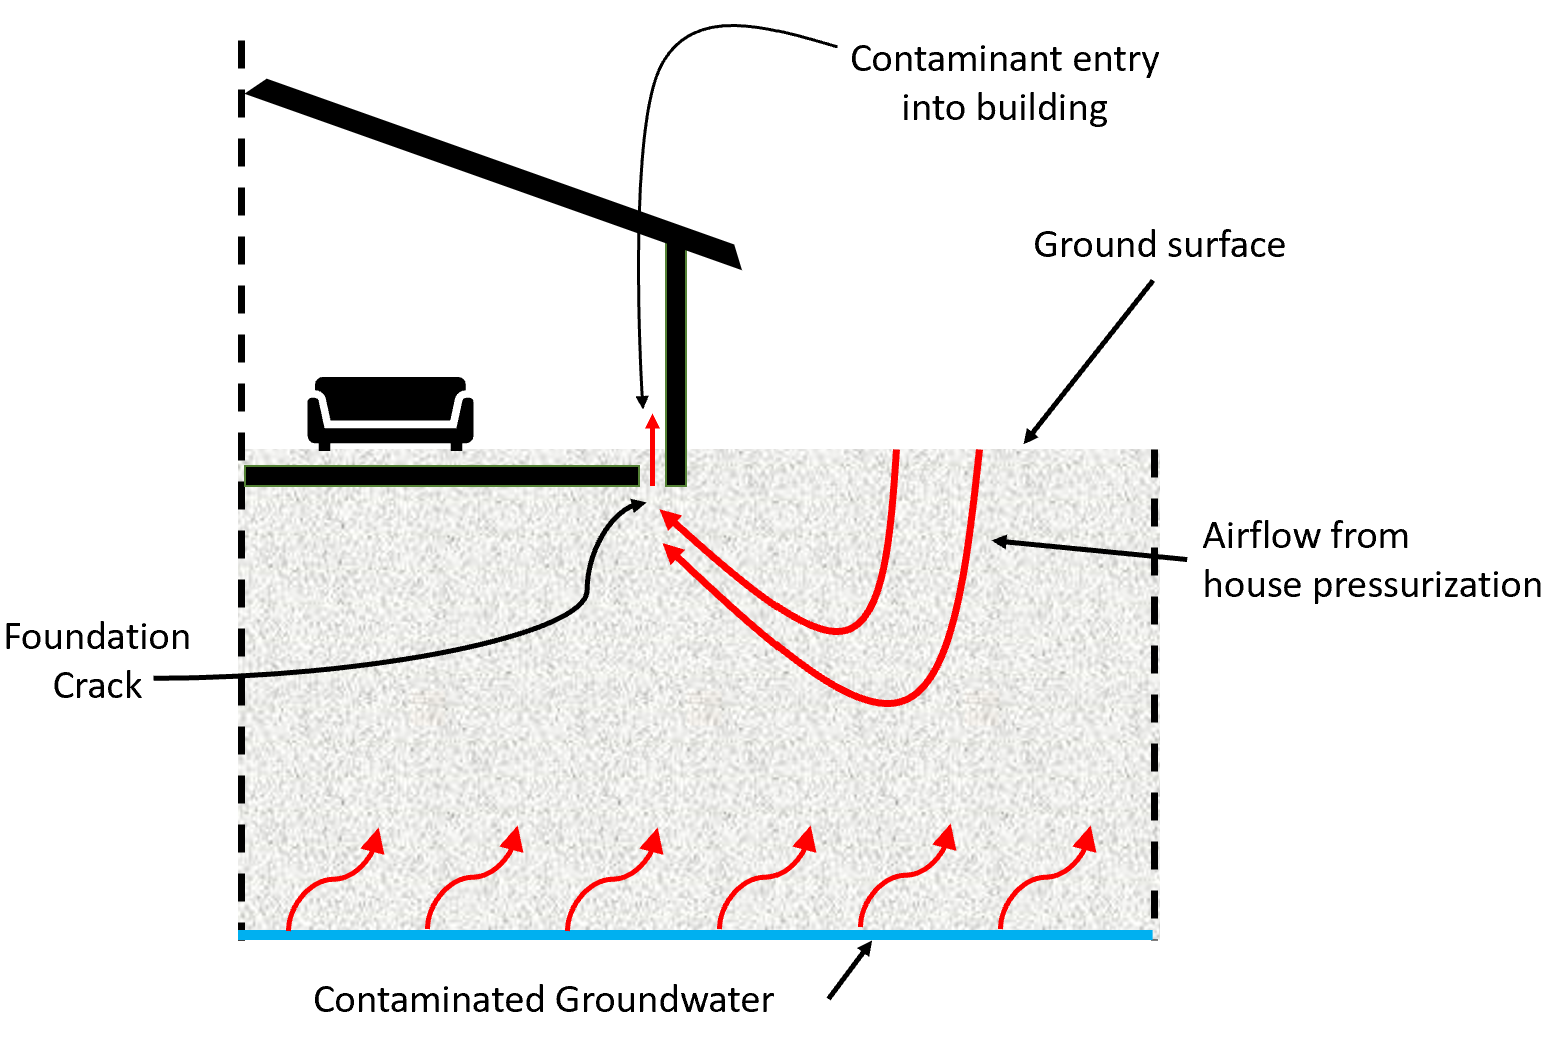
\includegraphics[width=0.75\textwidth]{model_cartoon.png}
  \caption{The considered VI scenario.}
  \label{fig:vi_scenario}
\end{figure}

The basement interior will be modeled as a continuously stirred tank reactor (CSTR), (but without reactions), where the indoor contaminant concentration will depend on the contaminant entry rate $n_\mathrm{ck}$ from the soil via the foundation crack and the air exchange rate $A_e$.
The details of this will be covered section \ref{sec:indoor}.\par

To determine $n_\mathrm{ck}$ the contaminant transport in the soil needs to be modeled.
This will be done using the advection-diffusion equation, which will be modified for transport in soils.
The contaminant transport itself is driven by a concentration gradient (leading to diffusive transport) and airflow (leading to advective transport) in the soil.
The contaminant source (groundwater) and sink (atmosphere and contaminant entry into the building) will largely determine the concentration gradient, while the airflow needs to be calculated separately.\par

The airflow in the soil is modeled by Darcy's Law, and is driven by a pressure gradient in the soil, which induced by the indoor/outdoor pressure difference at the interface between soil and building foundation.
Details are discussed in section \ref{sec:darcys_law}.\par

One last consideration is that the vadose zone is generally partially saturated with water, with the soil pores more or less water-filled near the groundwater interface, and with soil moisture content decreasing as a function of elevation above groundwater $z$ [\si{\metre}].
The soil moisture content has a profound effect on transport in the soil; it restricts both the airflow and contaminant diffusivity in the soil.
Thus, the soil moisture content $\theta_w$ must first be determined in order to solve the contaminant transport and Darcy's Law.\par

The resulting physical system is highly coupled, with many physical aspects dependant on others.
Figure \ref{fig:physics_overview} shows the coupling between each physicsal process, its output, and how it relates to the other processes that ultimately determine VI.\par

% TODO New figure
% TODO New caption + description
\begin{figure}[htb!]
  \centering
  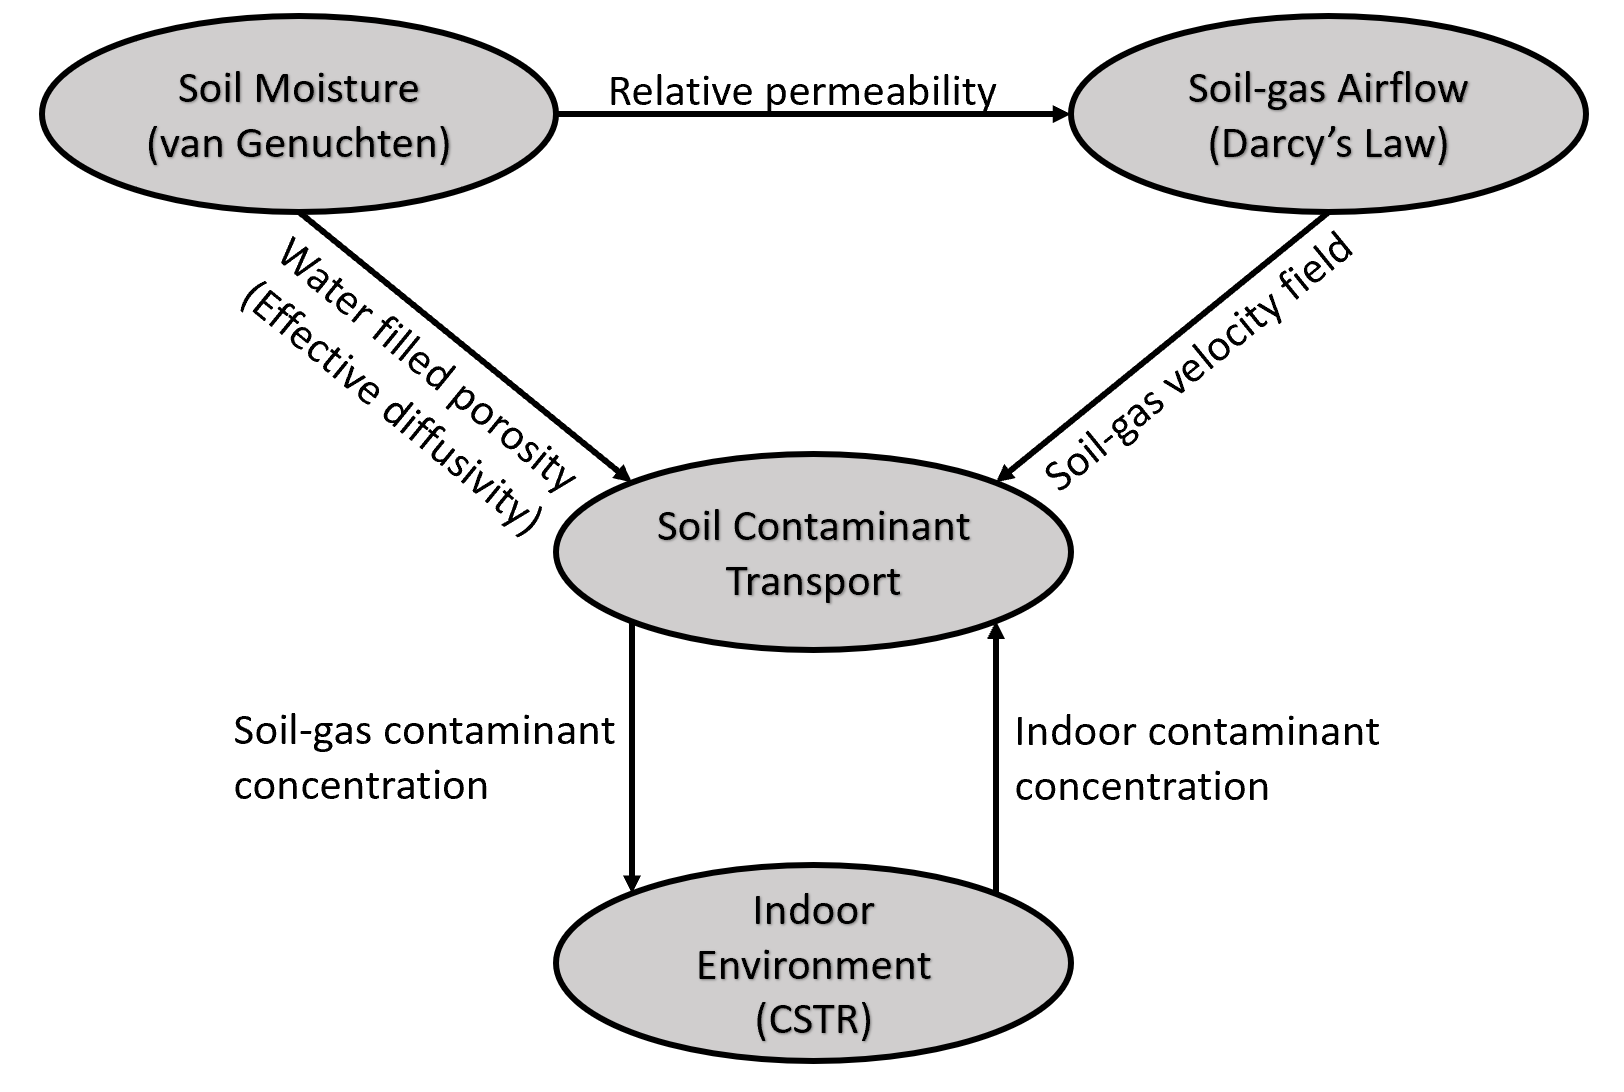
\includegraphics[width=\textwidth]{physics_interaction.png}
  \caption{Coupling between the physics used to model VI.}
  \label{fig:physics_overview}
\end{figure}

In this chapter, we will walk through the process of numerically modeling this VI scenario using the finite element method (FEM) and post-processing of the results.
A discussion regarding past and present VI models, their advantages and limitations, will follow.
Note that a particular numerical values cited above have been chosen to be "typical" of a VI scenario.
Clearly other values can be chosen for most of the parameters.
When results are presented below, the sensitivity of the results to particular parameter choices will be explored.\par
